\chapter{Conclusões}
\label{chap:conclusoes}

Neste capítulo são apresentadas as conclusões deste trabalho. Na
Seção~\ref{sec:c:resumo} é realizado um paralelo entre os objetivos desta tese
e os resultados obtidos. Na Seção~ \ref{sec:c:limitacoes} são discutidas
algumas limitações das soluções propostas e na Seção~\ref{sec:c:futuros} são
apresentadas algumas direções de trabalhos futuros.

\section{Resumo dos Objetivos e Principais Resultados}
\label{sec:c:resumo}

O objetivo principal deste trabalho foi apresentar a capacidade de aplicar camadas convolucionais para contar objetos em vídeos, considerando as posições dos mesmos no quadro anterior. Assim são estimados um mapa de densidade e a estimativa de deslocamento de alevino.

O melhor resultado obtido alcançou 98\% de acertos avaliados pela métrica F1, o que nos mostra que a técnica proposta se ajusta positivamente ao conjunto de dados. A métrica de erro MAE afirma que os equívocos cometidos pela rede em camadas é próximos a 0.
O objetivo de refinar o mapa de características utilizando os vetor de deslocamento foi alcançado visto que os melhores resultados se mostraram a partir do processamento das posições que precedem o quadro atual. 

\section{Limitações}
\label{sec:c:limitacoes}

Os alevinos estão em constante movimento nos vídeos, porém existem alguns peixes, geralmente dois(ou até mais) que se juntam e mantém um certo movimento uniforme confundindo a CNN, fazendo-a detectar apenas um peixe naquela posição na imagem. Como o deslocamento dos dois são análogos nos quadros anteriores $I_{t-1}$, no quadro atual $I_{t}$ processado não há possibilidade de se distinguir um do outro. O pico apontado pela CNN para estes peixes extremamente próximos é único e como a detecção é obtida através deles, a CNN detecta estes peixes como um. Na imagem \ref{fig:PeixesPróximos} temos um exemplo de dois peixes que se movimentam igualmente sem indicar uma desaproximação.

\begin{figure}[!ht]
	\centering
	
	\subfloat[quadro 187]{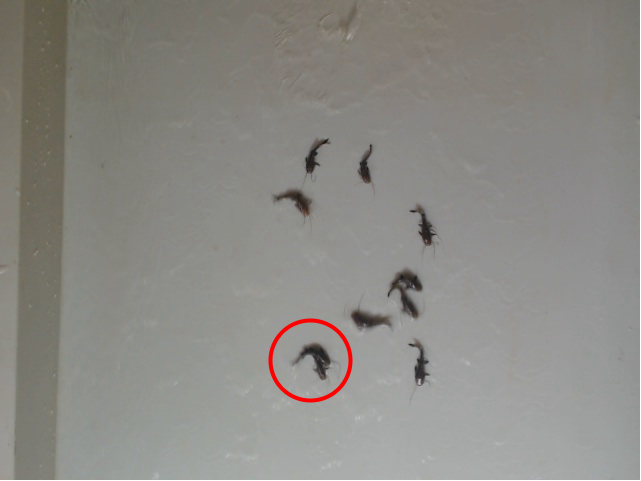
\includegraphics[width=0.46\textwidth]{image/187.png}}\vspace{0.2cm}
	\subfloat[quadro 188]{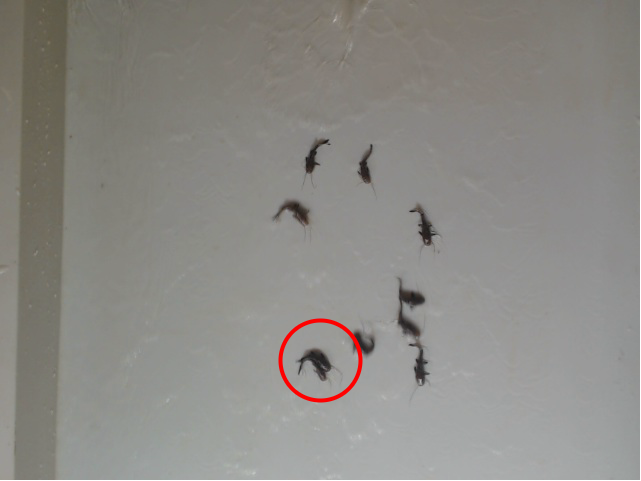
\includegraphics[width=0.46\textwidth]{image/188.png}}\vspace{0.2cm}

	\caption{\label{fig:PeixesPróximos} Exemplos dos peixes extremamente próximos que se movem uniformemente. Imagens do vídeo 06, quadro 187 e 188.
	%\textbf{TROCAR por IMAGENS da pasta "melhoresResultadosVisuais"}
	}
\end{figure}  

\section{Trabalhos Futuros}
\label{sec:c:futuros}

O fato de ocorrer peixes muito próximos nos faz entender que a técnica deverá abordar este tipo de situação. No qual serão testados técnicas para distinguir tais alevinos de maneira com que cada um seja detectado e somado a contagem final.

O método proposto será reavaliado em outro banco de imagens, para averiguar o potencial da técnica em detectar peixes em várias situações do mundo real. Nas imagens da Figura \ref{fig:proxbanco} temos amostras do banco a ser utilizado em novos experimentos.

\begin{figure}[!ht]
	\centering
	
	\subfloat[quadro 4810]{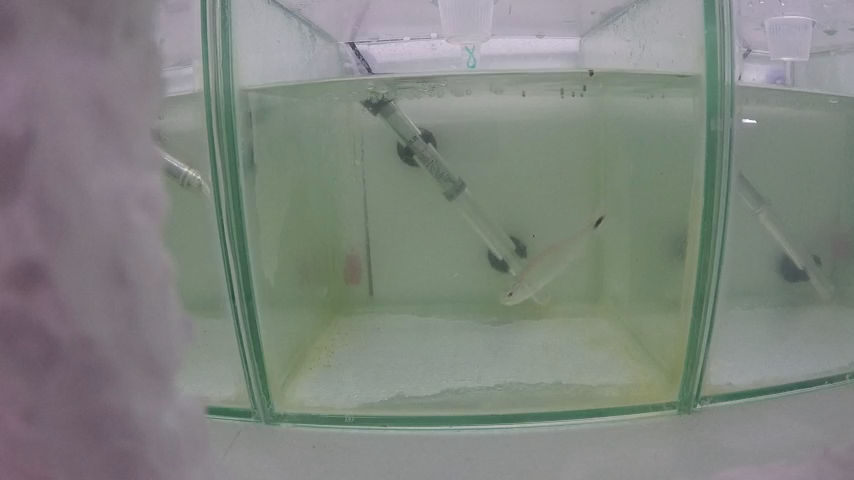
\includegraphics[width=0.8\textwidth]{image/frame0004810.png}}\vspace{0.2cm}
	\subfloat[quadro 6253]{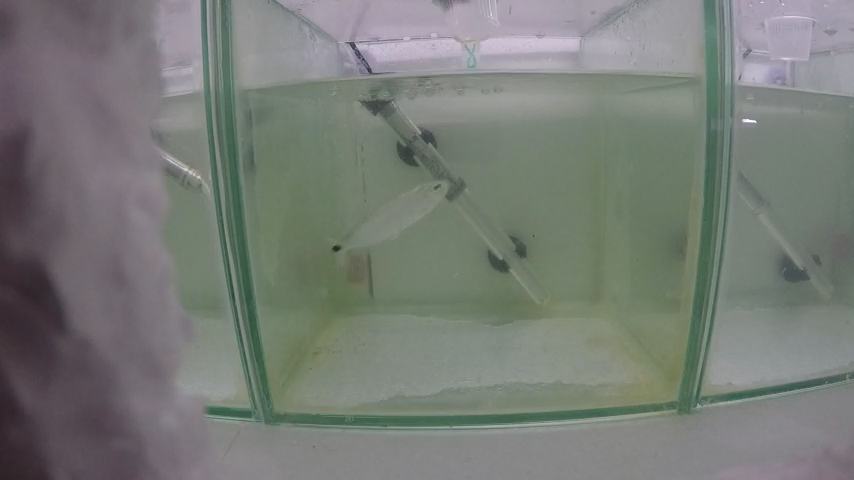
\includegraphics[width=0.8\textwidth]{image/frame0000247.png}}\vspace{0.2cm}

	\caption{\label{fig:proxbanco} Amostra do próximo banco de imagens a ser testado - vídeo 203.
	%\textbf{TROCAR por IMAGENS da pasta "melhoresResultadosVisuais"}
	.}
\end{figure}  

